
\documentclass[review]{elsarticle}
\usepackage{color}
\usepackage{lineno,hyperref}
\hypersetup{colorlinks, linkcolor=red}
\modulolinenumbers[5]

\journal{}

%%%%%%%%%%%%%%%%%%%%%%%
%% Elsevier bibliography styles
%%%%%%%%%%%%%%%%%%%%%%%
%% To change the style, put a % in front of the second line of the current style and
%% remove the % from the second line of the style you would like to use.
%%%%%%%%%%%%%%%%%%%%%%%

%% Numbered
%\bibliographystyle{model1-num-names}

%% Numbered without titles
%\bibliographystyle{model1a-num-names}

%% Harvard
%\bibliographystyle{model2-names.bst}\biboptions{authoryear}

%% Vancouver numbered
%\usepackage{numcompress}\bibliographystyle{model3-num-names}

%% Vancouver name/year
%\usepackage{numcompress}\bibliographystyle{model4-names}\biboptions{authoryear}

%% APA style
%\bibliographystyle{model5-names}\biboptions{authoryear}

%% AMA style
%\usepackage{numcompress}\bibliographystyle{model6-num-names}

%% `Elsevier LaTeX' style
\bibliographystyle{elsarticle-num}
%%%%%%%%%%%%%%%%%%%%%%%

\begin{document}

\begin{frontmatter}

\title{Results of brightness and uniformity measurements of various scintillator tiles at the CERN H2 test beam}


%% or include affiliations in footnotes:
\author[umd]{Alberto Belloni}
\author[umd]{Jeff Calderon}
\author[rochester]{Pawel De Barbaro}
\author[umd]{Sarah C. Eno}
\author[umd]{Geng-Yuan Jeng}
\author[umd]{Mahan Amouzegar}
\author[umd]{Yao Yao}

\address[umd]{Dept. Physics, U. Maryland, College Park MD 30742 USA}
\address[rochester]{The University of Rochester, Rochester, NY, USA}

\begin{abstract}
Radiation damage has been shown to reduce the overall output of scintillating material.
Not all materials, however, are as susceptible.
To subject the prototype liquid tile to realistic detector conditions, the test was conducted at the H3 Test Beam facility of CERN's Large Hadron Collider (LHC)complex. 
At the H2 site muons of specific energies are peeled away from the particle beam which approximate the conditions in which the Hadron calorimeter (HCAL) will actually function. 
In this way the H2 provides a “particle gun” which can be turned off and on for data acquisition. 
We collect our scintilator light output information using a Data Acquisition (DAQ) system designed for the phase one upgrade featuring Silicon Photomultipliers (SiPM). 
An attempt was made to compare the light yields, efficiencies, and uniformity of prototype liquid tiles and traditional plastic tiles. 
Here we present our finding and report upon the feasibility of liquid tile replacements to exiting plastic tiles.
\end{abstract}

\begin{keyword}
organic scintillator\sep liquid scintillator\sep radiation
hardness \sep calorimetry
\end{keyword}

\end{frontmatter}

\linenumbers

\section{Introduction}
\label{sec:introduction}
Run 2 began at The Compact Muon Solenoid (CMS) experiment at the Large Hadron Collider in summer of 2015. 
Research into the possibility of radiation resistant scintillators has shown that CMS presently has scintillators which are will degrade over time and cause photon re-absorption.
This will in turn cause the degradation of the output signals to the photomultiplier tubes, ultimately reducing the sensitivity of the CMS experiment. 
This degradation is expected to become increasingly sever in the near future due to the increased luminosity from upgrades performed prior to Run 2. 
This unavoidably exposes equipment to increasing levels of radiation. 
Plastic scintillators are particularly susceptible to this radiation and research is needed to find alternative technologies which will continue to function for the life of the machine. 
To that end, we conducted experiments aimed at comparing the light yield and efficiency of liquid scintillator prototypes.
The prototypes tested varied in design. One design featured a plastic-free liquid wave-length shifting capillary in place of traditional plastic wavelength shifting fibers, 
while another uses traditional plastic fibers. 
The plastic free design represents our fully radiation resistant solution.

\section{Experimental Area}
\label{sec:experimental_area}
This experiment was conducted at the H2 Beam Line located at the Prevessin site of the LHC complex.
The H2 Beam Line is part of the Super Proton Synchrotron (SPS). 
Since The SPS is capable of accelerating protons to 450 GeV it is useful for gauging the effectiveness of scintillators under realistic “Beam on” conditions. 
Magnets bend and focus the collimated beam directly onto a movable table.
The Table can move in all three dimensions allowing the user to align the target with the beam. 
This allows for gross output measurements of the scintillators as well as a means for ensuring our target is properly aligned. 
Since we wish to maximize the sensitive areas of our detector we need a proper alignment to ensure we have sufficient coverage over the area of the tile.    
Prior to reaching the table, the beam path passes through several instruments for precise tracking. 
In order of increasing distance from the beam pipe where the following instruments: 
wire chamber "A," 4 large scintillating plastic "paddles," wire chamber "B", wire chamber "C" and finally the movable table with the attached tiles. 
The uniformity measurement is made possible by the 3 wire chambers. 
After the beam exits the beam pipe it encounter the set of 100 by 100 millimeter electron drift chambers: wire chambers "A," "B," and "C." 
As the particles traverse the chambers the position of the particle is known to within a one half of a millimeter. 
The flow of electrons into the wires relay the position signature for each event and this information is stored along with the event number. 
The chambers also insure that the beam is properly aligned and focused. 
Each position registered on the wire chamber indicates a particles passing through the wire chamber. 
The aggregate position measurements are used to infer the trajectory of each muon and hence its intersection point with the tile. 
This position is matched with the signal pulse transmitted by the SiPM then to the rest of the data acquisition system. 
A histogram of the signal output would indicate the responsiveness of any region the tile.  
Because of the limitation of the wire chambers, this experiment kept the beam rates to $10^3$ particles per burst. 
Also we note that the highest efficiency region of the wire chambers is the 80 $mm^2$ center. 

%test beam area description, DAQ, trigger, tracking chambers...
\section{Scintillators}
\label{sec:scintillators}

The plastic tiles used were cut into 10\,cm x 10\,cm x 5\,mm squares. 
Each tile contained a sigma shaped groove. 
This grove holds a fiber which leads out of the tile and into a connector. 
The connector was shaped specifically to fit in a plastic case which houses each tile. 
This housing served the dual purpose of holding the sample in place and keeping outside light from effecting the scintillator measured output. 
The plastic connector rested between the two halves of the case. 
This connector is used to attach the wave length shifting fiber (WLS) from the tiles to the longer fiber optic transfer cable. 
These longer fibers lead to the optical device unit (odu). 
The ODU is part of the larger the Readout Module. 
The ODU contains 217 fiber connections which terminate at the face of yet more fibers which terminate on a battery of SiMPs arranged in a 6 x 8 array. 
Each SiMP transmits an electrical signals to the Front End Create where a series of Charge Integrator and Encoder (QIE10) chips are housed. 
These chips convert the along signal from the SiPMs to a digital signal integrated over a 25 nanosecond time window. 
The Front End Electronics (FEE) contain the alignment and formatting (FE-FPGA), the trigger-primitive and pipeline electronics (uHTR) and the cDAQ link (AMC13). 
From the front end electronics the data is transferred via  Gigabit Optical Link (GOL) to the back-end Electrons at 1.6 Gbps. 
A more detailed treatment on the electronics used in this set up can be found in CERN-LHCC-2012-015 / CMS-TDR-010 a technical design report. 

It is important to note that the triggering mechanism for this experiment differed from that of the technical design report. 
The triggering for the data acquisition system is accomplished by two scintillating paddles. 
These paddles are located between wire chamber "A" and "B" arranged one behind another in such a way that overlapping regions are perpendicular to the beam. 
Coinciding signals from both paddles result in a trigger condition. 
Of necessity we required a triggering mechanism which allows us to predict precisely when to expect muons to deposit their energy and register a hit in our efficiency calculation. 
For this analysis we had to calibrate our trigger such that data acquisition commences prior to the expected muon interaction time. 
This allows us to compare the interaction SiMP output to the background "dark current" signal. 
This "dark current" must be subtracted away from the total integrated charge, in this manner we can measure the true output signal. 
The plots which follow were produced by subtracting away the pedestal in this manner. 
\begin{figure}[!ht]
\begin{center}
  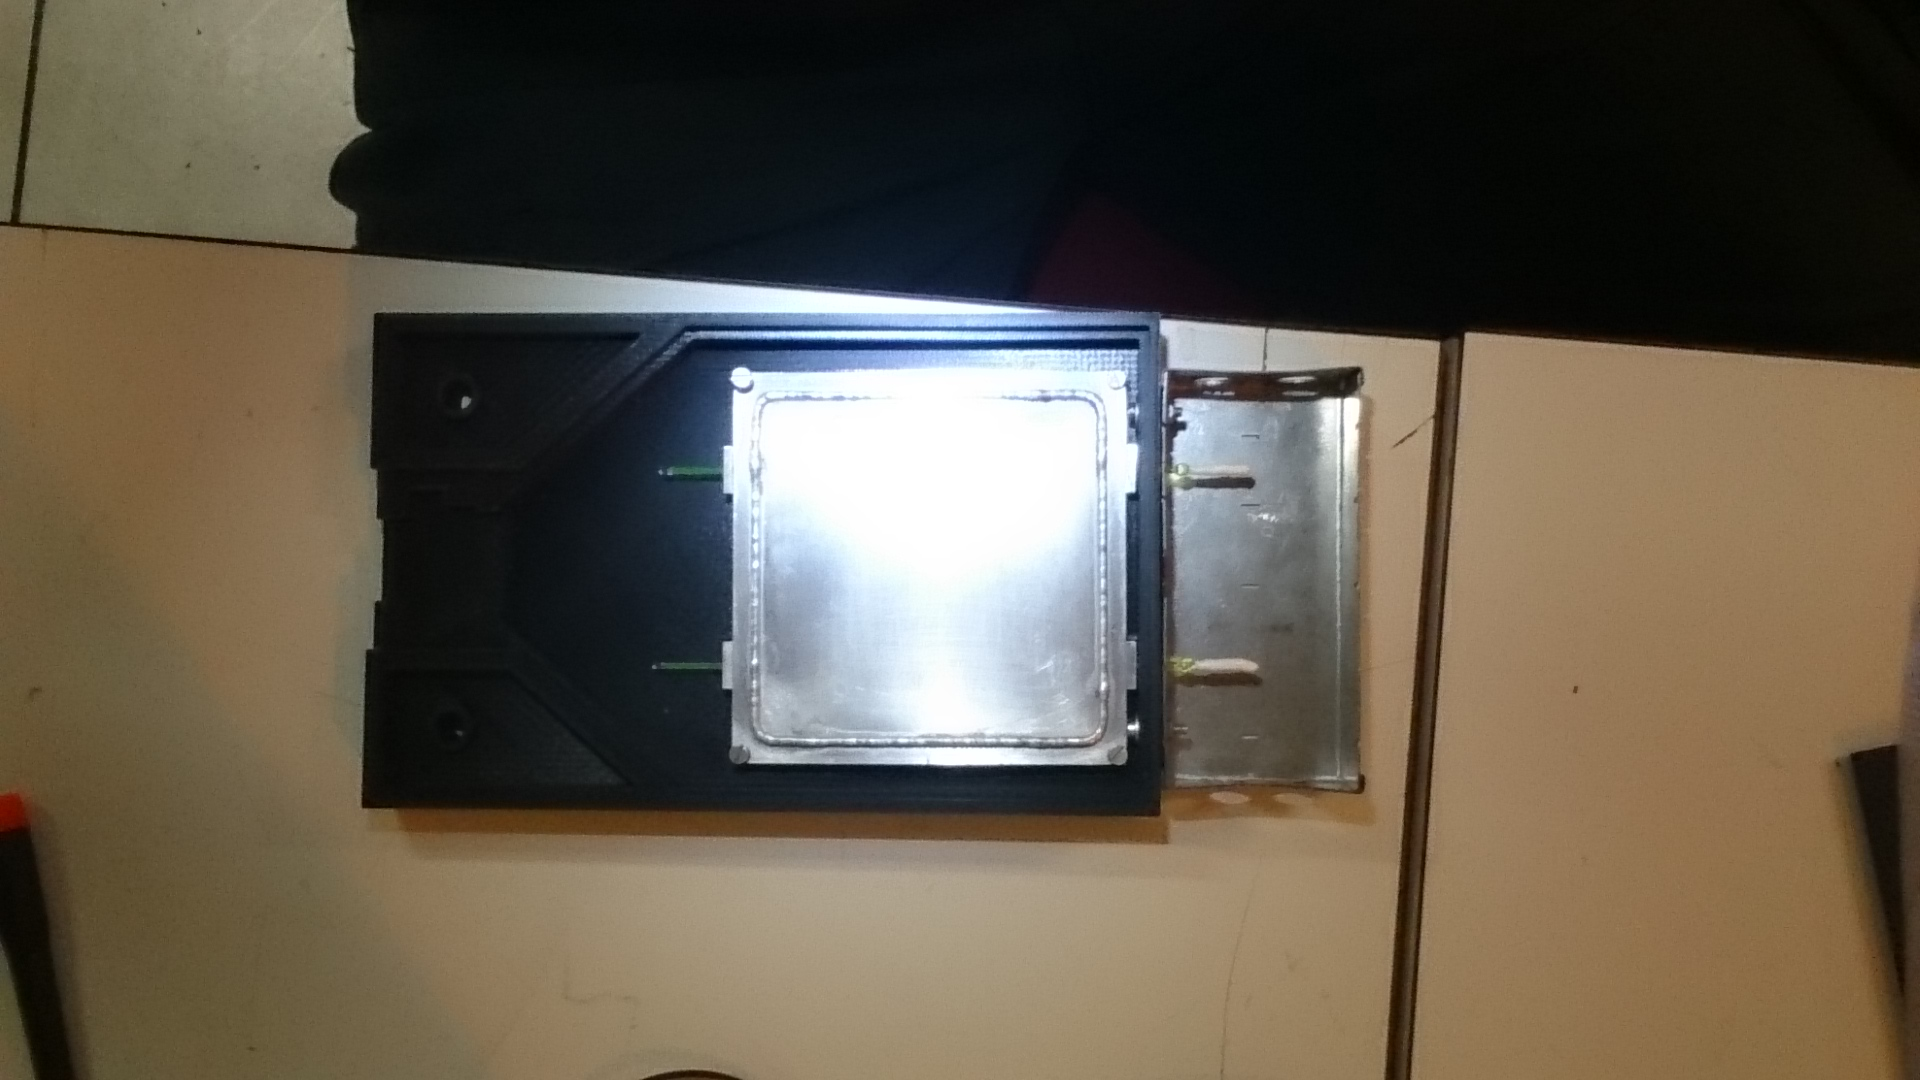
\includegraphics[width=1\textwidth]{./figures/qtile5.JPG}
\caption{Container for Aluminum tile with capillaries.}
}
\label{fig:capilary tile}
\end{center}
\end{figure}
Among the plastic scintillators tested are:
SCSN-81, EJ-260, EJ-309 and  EJ-200.
One of the tiles was made of SCSN-81. 
SCSN-81 is the blue-scintillating plastic having its peak emission around 440nm. 
It is manufactured by Kuraray which is presently used through out the CMS detector. 
This scintilator has a polyvinyltoluene as its base. 
The photons produced per MeV

EJ-200 has an emission spectrum which peaks around 425nm making it a blue scintillator. 
It has a Scintillation effieciency of 10000 photons per MeV.
It has Polyvinyltoluene base material and is produced by Eljen Technology. 
It is similar to BC-408 which is used in the first layer of the CMS calorimeter.

EJ-260 is a standard industrial plastic scintillator made of the same polyvinyltoluene base as EJ-200.
It's emissions spectrum reaches a peak around 490nm making EJ-260 a green scintillator. 
It has a Scintillation effieciency of 9200 photons per MeV.

The liquid  Scintillator material used in this experiment was EJ-309. 

EJ-309 is a xylene based scintillator.
It has a Scintillation effieciency of 11500 photons per MeV.
EJ-309 is also made by Eljen Technology and features a higher flash point than previous liquids, while presevering comparable light emmission.
It has a peak at around 425nm. 
More information on EJ-309 can be found at Eljen's website: \url{http://www.eljentechnology.com} 

Two separate Aluminum tiles were prepared. 
One with quartz support tubes running through the liquid to hold 1\,mm Y-11 WLS fiber.
The WLS fiber is manufactured by Kuraray and has its emission peak at 476nm. 
Another Aluminum tile was prepared which had liquid capillaries containing a liquid wavelength shifting material rather than Y-11 fiber. 
Like Y-11, the liquid the shifts blue scintillator light into the blue frequency range. 
Prior to mounting the special care was taken to pour the liquid scintillator  into our aluminum tiles under nitrogen environment as oxygen.
Details on the tiles can be found in \cite{mdliquidtile}.


\begin{figure}[!ht]
\begin{center}
  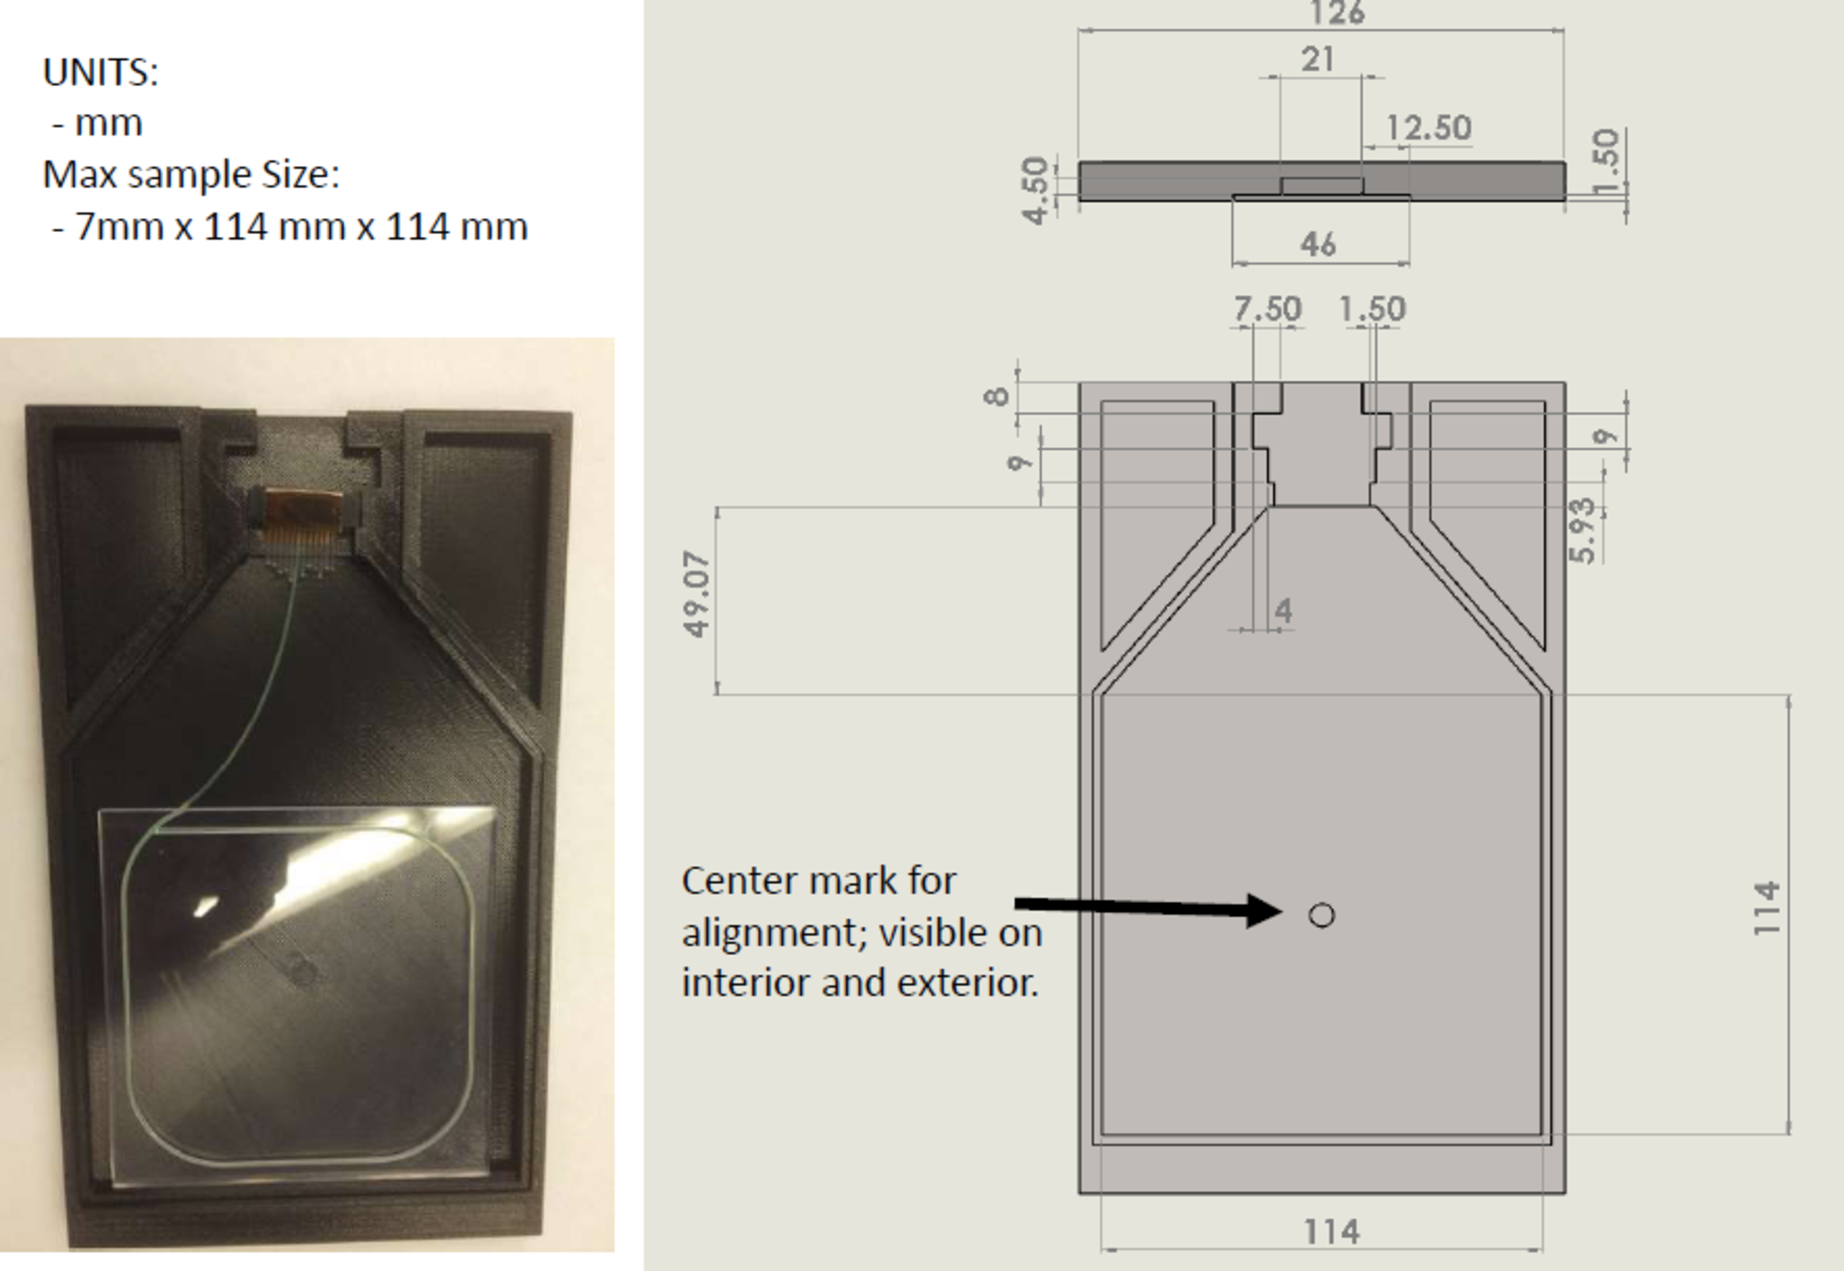
\includegraphics[width=1\textwidth]{./figures/samplemount.pdf}
\caption{Container for plastic tiles.}

\label{fig:capilary tile}
\end{center}
\end{figure}

Details on the tiles can be found in~\cite{mdliquidtile}.

\section{Data Samples}
\label{sec:data_samples}


\section{Energy Analysis}

%energy, efficiencies...
%PLOTS TO INCLUDE: 
%energy (entries vs ADC counts)
% entries vs x and y (i.e., map of the beaam spot)
%efficiency vs x and y, efficiency vs x, efficiency vs y

\section{Time Analysis}

%timing plots: I have the plots (ask me for them)
%PLOTS: deltaT between EJ-260 rising edge and SCSN-81 rising edge, EJ-200 vs SCSN-81

\section{Conclusion}





\section{Acknowledgments}
The authors would like to thank Randy Ruchti of Notre Dame for
providing the capillaries. 
Grant DESC0010072.

\section*{References}

\bibliography{testbeam}

\end{document}
